\bookchapter{第三十七章：パラダイム革命——「コードを書く」から「AI にコードを書かせる」へ}

\chapterintro{おめでとうございます。この本を開いたあなたは、いま職業のパラダイム革命のど真ん中に立っています。この革命の起点は、2025年に一人のプログラマーが SNS に投稿したひと言でした。少しドラマチックに聞こえますか？でも、本当にあったことです。}

\booksection{Vibe Coding の誕生：ひと言が引き起こしたムーブメント}

2025年2月、Andrej Karpathy——この名前は今のうちに覚えておいてください。この先も何度も登場します——が、後になって繰り返し引用されることになった投稿を SNS に上げました：「Vibe Coding という新しいプログラミングのやり方がある。完全にフィーリング（vibes）で進めて、コードの細かいところは気にせず、AI に全部まかせる。見えたものをそのまま口にして、コピーアンドペースト、だいたい動けばそれでいい。」

とりとめのない独り言に見えるこの発言は、実はすでに静かに起きていたパラダイムシフトに、ぴったりの名前を与えたのです：人間はもうコードを1行ずつ書かず、自然言語で意図を記述し、AI が実装を完成させる。Karpathy の言い回しには少し揶揄の色がありましたが、その背後には深い洞察があります：AI のコード生成能力がある閾値を超えたとき、プログラミングのボトルネックは「この行のコードが書けるか」ではなく「この件を自分ははっきり考えられているか」に変わるのです。

\begin{tcbinfo}{ヒント：Vibe とは何？}
Vibe を直訳すると「雰囲気、フィーリング」。Vibe Coding とは「感覚に従って AI にプログラミングを指揮させる」こと——あなたは欲しいものを記述し、AI が実装を担います。この言葉を覚えておいてください。この革命の「出生証明書」なのですから。

\end{tcbinfo}

あの瞬間から、「コーディング」という言葉の意味が分かれ始めました：従来のコーディングは、設計を文法に翻訳すること。新しいコーディングは、意図を指示に翻訳することです。前者は指が試され、後者は頭が試されます。

Vibe Coding という言葉は、すぐに冗談めいたものから真面目なエンジニアリングの概念へと変わっていきました。2026年半ばまでに、SNS 上のネタから、要件の表現、コンテキスト管理、反復検証、品質保証までをカバーする全プロセスを備えた、完全な方法論の体系へと進化しています。人々は同時に気づきました：「感覚でやる」のは入門段階の状態にすぎず、本当に効率的な AI プログラミングには、体系化された思考の枠組みが必要なのだと。そしてその思考の枠組みこそ、本書があなたに差し出すものです。

\booksection{2026年の現在地：Agentic Engineering の時代}

2026年8月に至るまでに、AI プログラミングの分野は、いくつもの重要なパラダイムの更新をくぐり抜けてきました。Vibe Coding は最初の火種でしたが、ほどなく皆が気づきます：「感覚のまま」AI とおしゃべりしているだけでは、生まれてくるコードの品質が極めて不安定——ときには感動的にうまくいき、ときには大失敗する。そこでパラダイムは進化し始めました：単純な対話型プログラミングから、構造化された Agent エンジニアリングへ。

またしても Karpathy です。2026年初頭、Agentic Engineering という概念を提唱しました。Vibe Coding の「言えば生成する」とは違って、Agentic Engineering が重視するのは：AI に目標を与え、ステップの計画、ツールの呼び出し、結果の検証、反復修正を自律的に行わせること。AI はもはや単なるコード生成器ではなく、環境を感じ取り、判断を下し、行動を実行できるインテリジェントなエージェント（Agent）なのです。

この転換は、3つの重要な変化をもたらしました：

\begin{enumerate}
  \item やり取りの形が変わった：「一問一答」から「目標を設定して権限をゆだねる」へ。
  \item 仕事の成果物が変わった：「コードの一片」から「完成したプロジェクト一式」へ。
  \item 人の役割が変わった：「コードを1行ずつレビューする」から「境界線を定め、結果を検収する」へ。
\end{enumerate}

数字は嘘をつきません：Cursor は2026年4月にリリースされた Cursor 3 で、Agent モードの使用率が初めて Tab 補完モードを追い越しました。開発者が大規模にこの働き方へ移行した証拠です。また、ターミナルネイティブの AI プログラミングツール Claude Code は、2026年半ばまでに年間換算で25億ドルの収入規模に達しました。次のトレンドグラフで、この交差の瞬間を直感的につかんでください：

\begin{center}
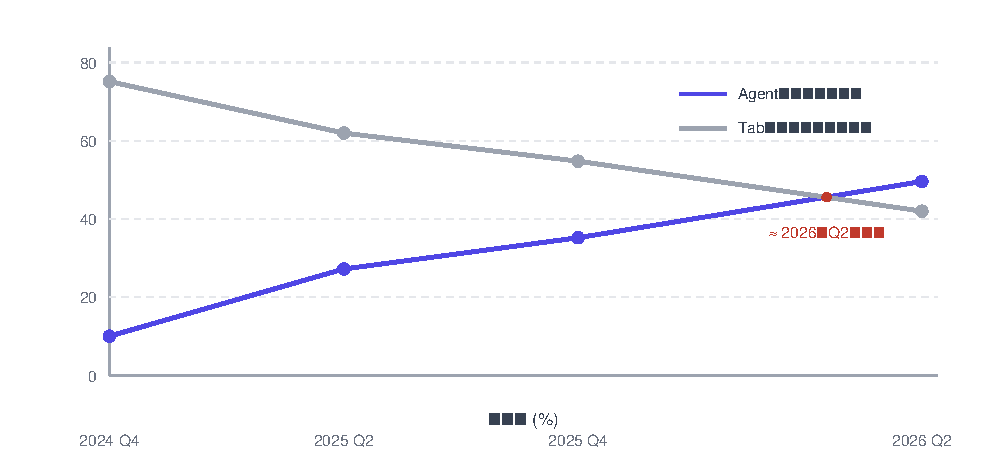
\includegraphics[width=0.92\linewidth]{figures/fig-di-san-shi-qi-zhang-1}
\\[2pt]\small 図1：AI プログラミングの対話モード使用率の変化（業界調査データに基づく推定。2026年 Q2 に Agent モードが Tab 補完を逆転）
\end{center}

でも正直に言いましょう：ツールとモデルの変化は、見えている表面にすぎません。Cursor を使おうが Claude Code を使おうが、土台のモデルが GPT-5 だろうと Claude 4.5 だろうと、成功している AI プログラミング実践者は皆、同じ一連の根本的な方法論に従っています。このガイドが教えるのは、まさにその部分です。

\booksection{核心となる認識の転換：Coder から Conductor へ}

従来のプログラミング教育は、Coder になる方法を教えます——文法を理解し、API を暗記し、ロジックの誤りを直す。AI プログラミングの時代には、この役割が再定義されつつあります。もうすべてのコードを自分の手で書く必要はありませんが、あなたは「指揮官」になる必要があります：戦場を定め、ルールをつくり、タスクを割り振り、成果を検収する Conductor です。

この転換の核心は「コードが書けるかどうか」ではなく、「何をしたいのかをはっきり考えられるかどうか」にあります。優れた指揮官は、必ずしも最良の兵士ではありません。しかし、戦いの目標·地形·兵力配置を誰よりもよく知っていなければなりません。同じように、優れた AI プログラミング実践者は、あらゆる言語の文法の細部に精通している必要はありません。しかし、プロジェクトの目標·アーキテクチャ上の制約·品質基準を誰よりもよく把握していなければなりません。

この表は2度見返す価値があります——今回の役割転換の全体像が、ここにまとまっているのです：

\begin{center}
\begin{tabularx}{\linewidth}{|X|X|X|}
\hline
\textbf{観点} & \textbf{従来の Coder} & \textbf{AI 指揮官（Conductor）} \tabularnewline
\hline
中核スキル & 文法の暗記、API の呼び出し、デバッグ & 要件の定義、コンテキスト管理、検収の判断 \tabularnewline
働き方 & コードを1行ずつ書く & 意図を記述し、成果物を審査する \tabularnewline
品質管理 & 自分で書いたコードの中身は、自分が一番わかっている & テストとレビューでAIの成果物を検証する \tabularnewline
求められる知識 & 特定の言語／フレームワークを深く習得する & 技術の全体像を広く、業務ロジックを深く理解する \tabularnewline
ボトルネックはどこか & コーディングの速さと文法の暗記 & 思考の明確さと表現力 \tabularnewline
エラーの原因 & 文法ミス、ロジックの抜け漏れ & 要件があいまい、文脈情報が足りない \tabularnewline
\hline
\end{tabularx}
\end{center}

\begin{center}\small\color{gray}従来のCoderとAI指揮官の能力の比較\end{center}

これは決して、プログラミングの知識が重要でなくなったという意味ではありません。むしろ逆です：AIが書いたコードが読めるからこそ、効果的にレビューして修正できます。データ構造とアルゴリズムを理解しているからこそ、AIの提案が妥当かどうか判断できます。知識の蓄積はあなたの「指揮の上限」を決めます——ただし知識の役割は、「実行の道具」から「判断のよりどころ」へと変わったのです。

\booksection{四、なぜ方法論がツールより大事なのか}

ツールは3か月ごとに改良され、方法論は3年ごとに進化します。ツールの操作を覚えても3か月後には古くなるかもしれない。けれど一つの考え方を身につければ、3年後もまだ使える。

AIプログラミングを始めたばかりの多くの人は、最初に「どのツールが一番良いか」「どのモデルが一番強いか」と問い立てます。これらの質問が大事でないわけではありませんが、優先順位を間違えています。2026年8月のツールの情勢は、2025年8月とはすでにまったく違います——TraeやQoderなどのツールは栄枯盛衰を繰り返し、Cursorはプラグインから独立したIDEになり、さらにCursor 3へ進化し、Claude Codeは実験的なプロジェクトからターミナルプログラミングの主流の選択肢になりました。しかし、この激しい変化の裏側で、成功している実践者たちが従っている思考の原則は、ほとんど変わっていません。

だからこそ本書は、特定のツールの具体的な操作を教えることに紙幅を割きません——そうした内容は書き終えた瞬間に古くなるからです。その代わり、本書のすべての重心は、検証ずみの思考方法論というひとつの体系に置かれています：要件をどう考えるか、AIとどうやり取りするか、成果物をどう検証するか、どう反復し続けるか。この方法論を身につければ、どのツールに変わってもすぐ使いこなせます。ツールの操作だけを学んだ人は、ツールが変わるたびにゼロからやり直しです。

\begin{tcbinfo}{ゼロベースの読者への安心材料}
ゼロから始める人は、「方法論」という三文字におびえないでください。方法論は抽象的な哲学ではなく、「問題に出会ったときどう考えるか」という操作マニュアルです。料理を学ぶのと同じです：レシピどおりに一歩一歩進めることもできます（ツールの操作）が、ほんとうの料理人は「なぜこの味付けなのか」「火加減をどう調整するのか」（方法論）を理解しています。本書はいちばん基本の概念から説明し、原則ごとに具体的な比較例を付けているので、「何か」がわかるだけでなく、「どうやるか」まで身につきます。

\end{tcbinfo}

\begin{tcbpractice}{やってみよう：いまの自分の「役割写真」を一枚撮ろう}
紙を一枚取り出して、三つの質問の答えを書きましょう：(1) いまはAIにどうやってコードを書かせているか（使ったことがあれば）？(2) 自分は上の表の「Coder」に近いか、それとも「指揮官」に近いか？(3) 三か月後の自分には、自分の働き方をどう表現してほしいか？書き終えたら本に挟んでおき、第四十七章を読み終えたらもう一度見返してください——変化は想像より速いと気づくはずです。

\end{tcbpractice}

\begin{tcbsummary}{本章のまとめ}
\begin{itemize}
  \item 2025年、KarpathyはAIプログラミング革命に「Vibe Coding」という名前を付けました：1行ずつコードを書くやり方から、自然言語で意図を記述するやり方へ
  \item 2026年にはAgentic Engineeringへ進化：目標を与え、権限をゆだね、AIが自律的に計画·実行し、人は成果の受け入れを担当
  \item Cursor 3ではAgentモードの利用率が初めてTab補完を追い越し、Claude Codeの年間収益は25億米ドルに達しました
  \item あなたの新しい役割はConductor（指揮官）：戦場を定め、ルールを決め、タスクを割り振り、成果を受け入れる
  \item ツールは3か月ごとに更新され、方法論は3年かけてしか進化しない——学ぶのは方法論であって、操作ではない
\end{itemize}

\end{tcbsummary}
